\documentclass{beamer}
\usepackage{animate}
\newcommand{\comment}[1]{}

% Load Packages
\usepackage[utf8]{inputenc}
\usepackage{xcolor}
\usepackage{tikz}
\usetikzlibrary{positioning,calc}
\usepackage{graphicx}
\usepackage{hyperref}
\usepackage{amsmath}
\usepackage{listings}
%\usepackage{fontawesome}

% Define Commands
\newcommand*{\ClipSep}{0.06cm} %To adjust footer logo
\newcommand{\E}{\mathrm{e}\,} %\def\I{e} % used to defined e for exp(x), see later what it should be
\newcommand{\ud}{\mathrm{d}}
\lstset{numbers=left, numberstyle=\tiny, stepnumber=1,firstnumber=1,breaklines=true,
    numbersep=5pt,language=Python,
    stringstyle=\ttfamily,
    basicstyle=\footnotesize, 
    showstringspaces=false
}

\usetheme{oxonian}

\title{LXe scintillation model}
\begin{document}

{\setbeamertemplate{footline}{} 
\frame{\titlepage}}

\begin{frame}{Objective}
The goal is is build a scintillation model for LXe: $Y_{a}(t,\hat{\theta})$.\\
$Y_{a}(t,\hat{\theta})$ is the probability to emit a photon at time $t$ to the direction $\hat{\theta}$. The subscript $a$ indicates the different type of interactions ($\gamma$, $N$, $\alpha$ and maybe different energies in the same interaction type).\\
\end{frame}


\begin{frame}{Signal Reconstruction}
%	\begin{center}
%	\animategraphics[loop,controls,width=0.6\linewidth]{10}{recon-}{0}{41}	
%	\end{center}
To study the temporal structure of the photon emission a processing algorithm uses a template of the average SPE signal to reconstruct the temporal PE pattern in each event for each PMT separately. The output of this process is the number of PEs created in the PMT in each digitization point.

\begin{figure}[h]
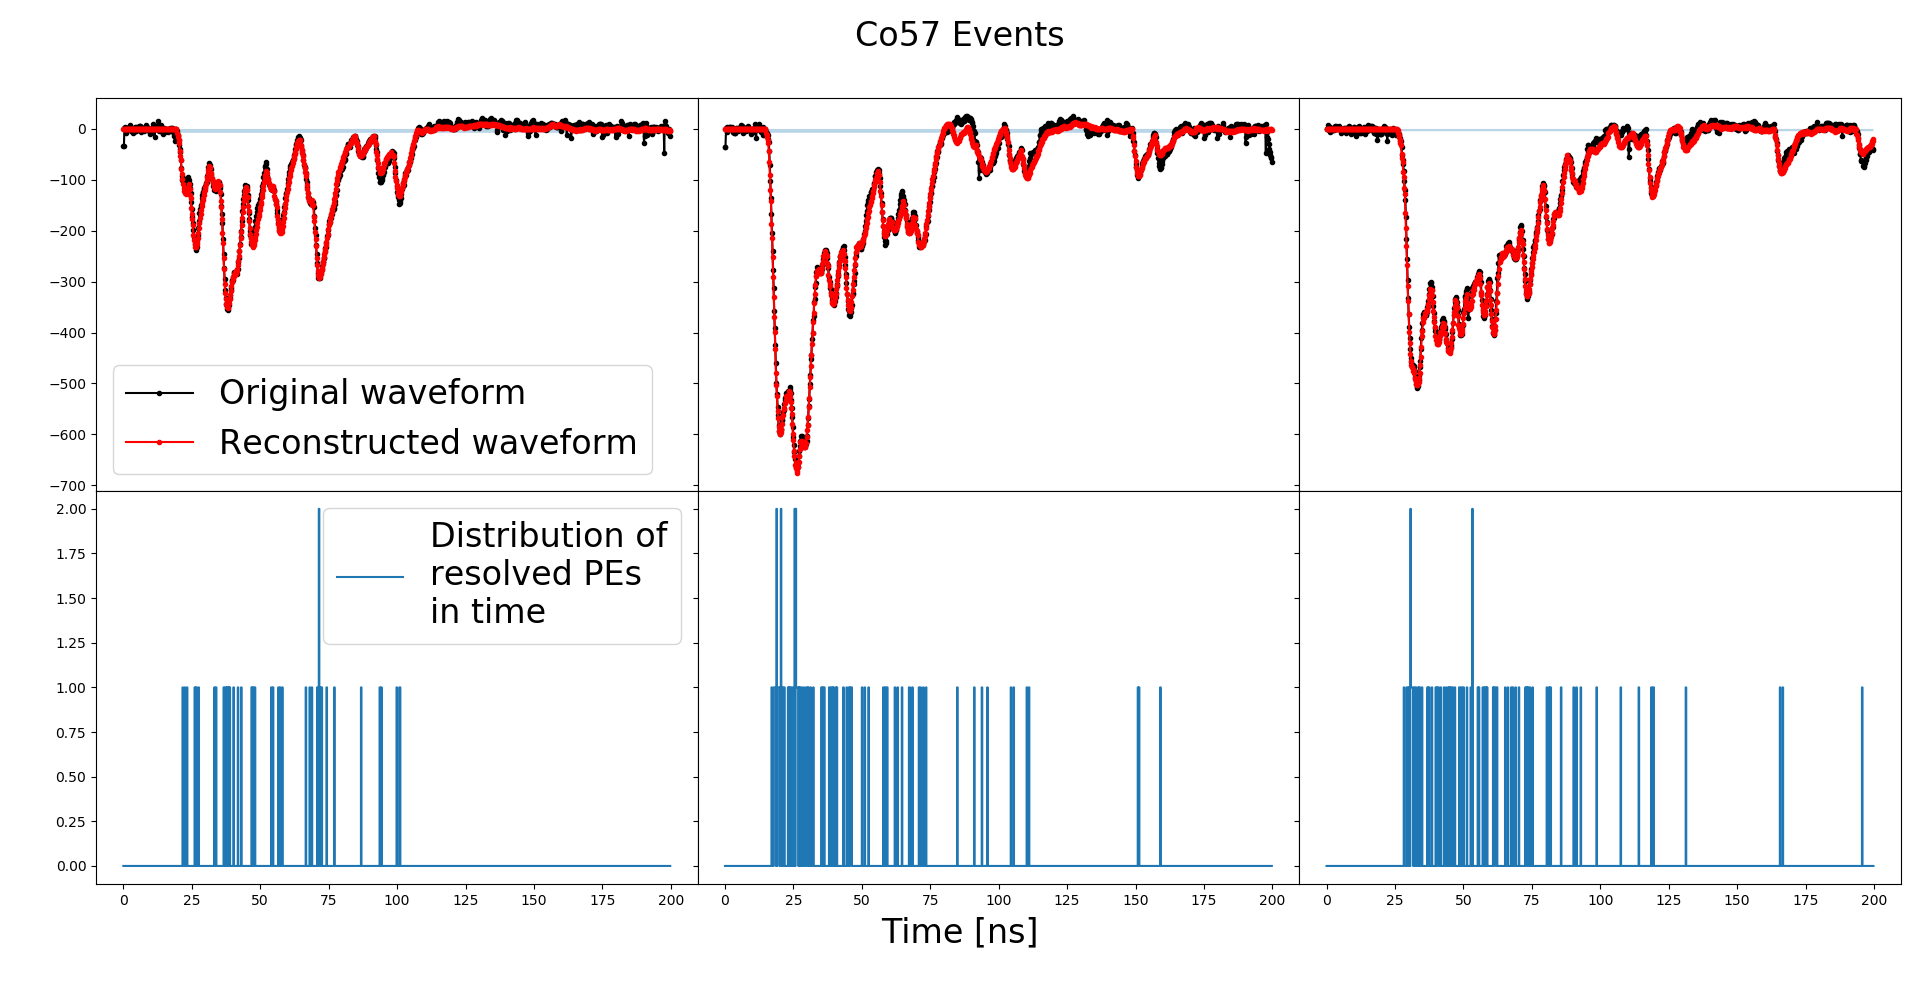
\includegraphics[width=1\textwidth]{recons.png}
\end{figure}

\end{frame}


\begin{frame}{Time Alignment Problem}
We do not know the "time zero" for each event due to two reasons:\\
\begin{itemize}
\item The trigger time is random so alignment by the trigger time would not help (align by the first resolved photon - second problem).
\item The resolved PEs time distribution is a sample of the times of the emitted photons and we don't know the delay between the first resolved PE and the first photon that was emitted.
\end{itemize}
\begin{figure}[h]
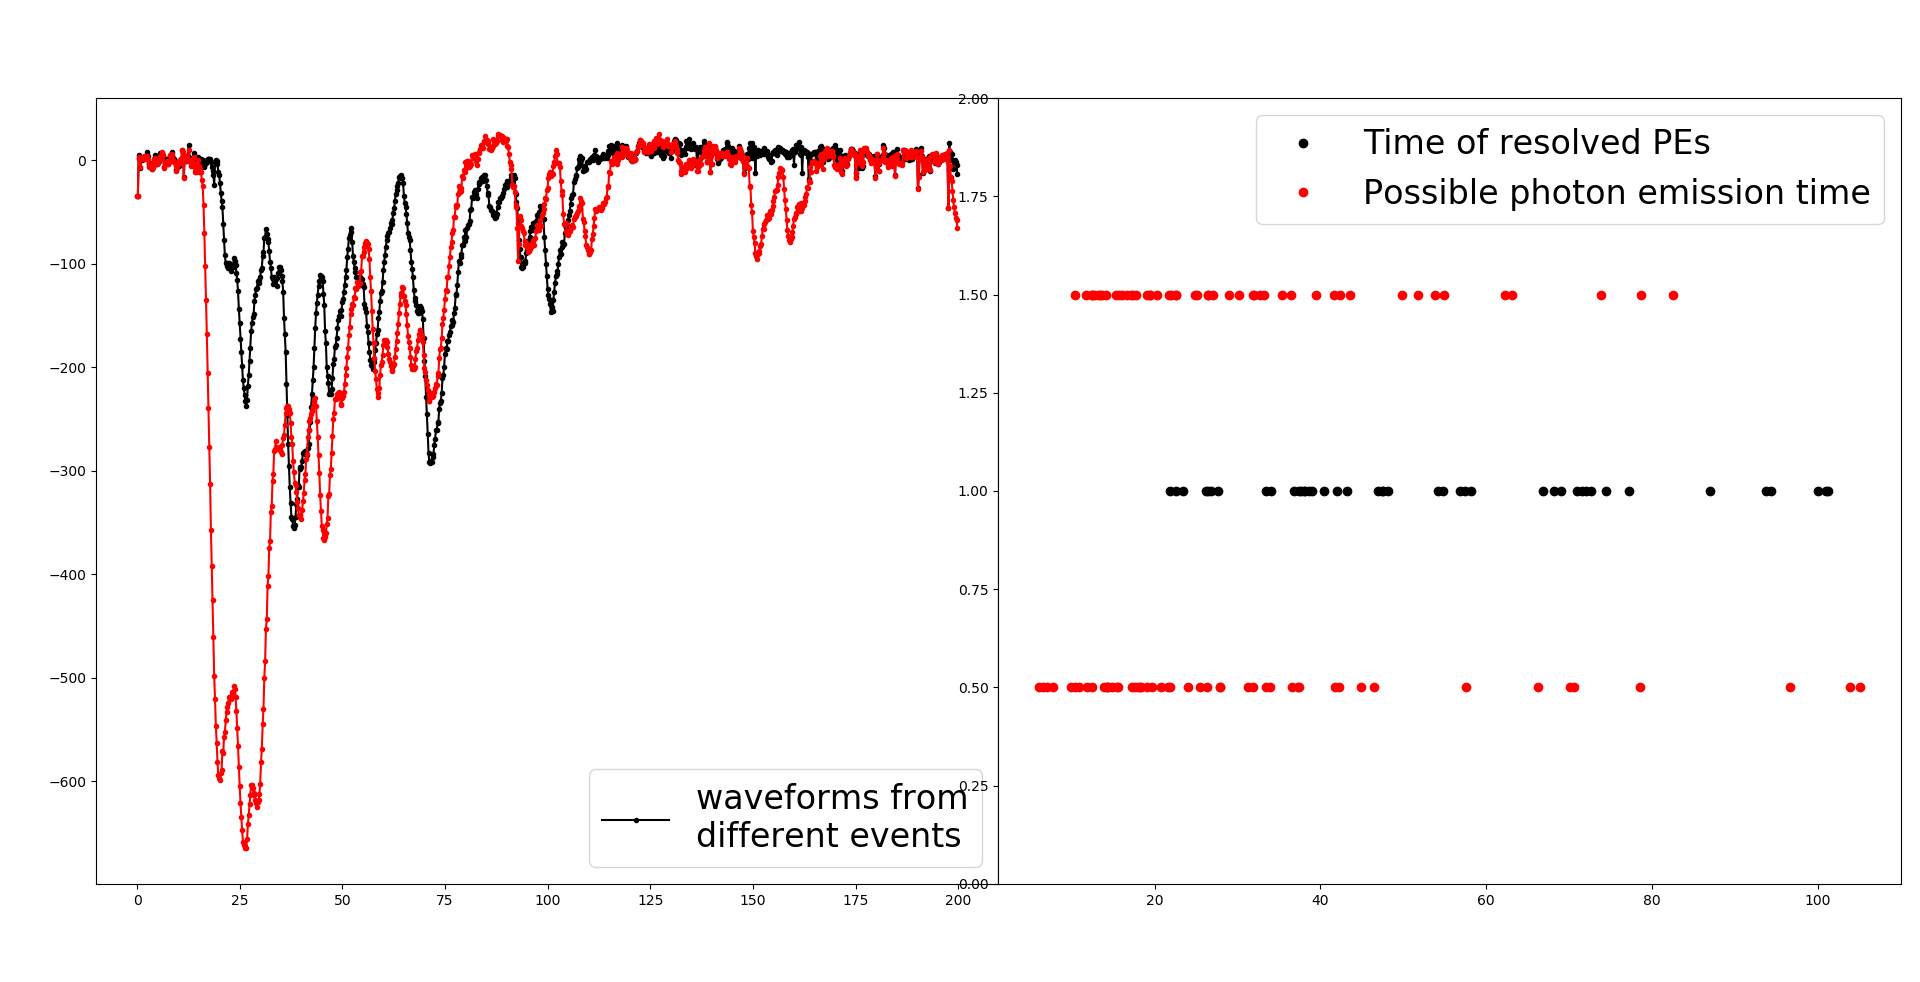
\includegraphics[width=0.5\textwidth]{alignment.png}
\end{figure}
Solution: Align by the first resolved photon and adjust the model.  
\end{frame}


\end{document}

